\documentclass[1p]{elsarticle_modified}
%\bibliographystyle{elsarticle-num}

%\usepackage[colorlinks]{hyperref}
%\usepackage{abbrmath_seonhwa} %\Abb, \Ascr, \Acal ,\Abf, \Afrak
\usepackage{amsfonts}
\usepackage{amssymb}
\usepackage{amsmath}
\usepackage{amsthm}
\usepackage{scalefnt}
\usepackage{amsbsy}
\usepackage{kotex}
\usepackage{caption}
\usepackage{subfig}
\usepackage{color}
\usepackage{graphicx}
\usepackage{xcolor} %% white, black, red, green, blue, cyan, magenta, yellow
\usepackage{float}
\usepackage{setspace}
\usepackage{hyperref}

\usepackage{tikz}
\usetikzlibrary{arrows}

\usepackage{multirow}
\usepackage{array} % fixed length table
\usepackage{hhline}

%%%%%%%%%%%%%%%%%%%%%
\makeatletter
\renewcommand*\env@matrix[1][\arraystretch]{%
	\edef\arraystretch{#1}%
	\hskip -\arraycolsep
	\let\@ifnextchar\new@ifnextchar
	\array{*\c@MaxMatrixCols c}}
\makeatother %https://tex.stackexchange.com/questions/14071/how-can-i-increase-the-line-spacing-in-a-matrix
%%%%%%%%%%%%%%%

\usepackage[normalem]{ulem}

\newcommand{\msout}[1]{\ifmmode\text{\sout{\ensuremath{#1}}}\else\sout{#1}\fi}
%SOURCE: \msout is \stkout macro in https://tex.stackexchange.com/questions/20609/strikeout-in-math-mode

\newcommand{\cancel}[1]{
	\ifmmode
	{\color{red}\msout{#1}}
	\else
	{\color{red}\sout{#1}}
	\fi
}

\newcommand{\add}[1]{
	{\color{blue}\uwave{#1}}
}

\newcommand{\replace}[2]{
	\ifmmode
	{\color{red}\msout{#1}}{\color{blue}\uwave{#2}}
	\else
	{\color{red}\sout{#1}}{\color{blue}\uwave{#2}}
	\fi
}

\newcommand{\Sol}{\mathcal{S}} %segment
\newcommand{\D}{D} %diagram
\newcommand{\A}{\mathcal{A}} %arc


%%%%%%%%%%%%%%%%%%%%%%%%%%%%%5 test

\def\sl{\operatorname{\textup{SL}}(2,\Cbb)}
\def\psl{\operatorname{\textup{PSL}}(2,\Cbb)}
\def\quan{\mkern 1mu \triangleright \mkern 1mu}

\theoremstyle{definition}
\newtheorem{thm}{Theorem}[section]
\newtheorem{prop}[thm]{Proposition}
\newtheorem{lem}[thm]{Lemma}
\newtheorem{ques}[thm]{Question}
\newtheorem{cor}[thm]{Corollary}
\newtheorem{defn}[thm]{Definition}
\newtheorem{exam}[thm]{Example}
\newtheorem{rmk}[thm]{Remark}
\newtheorem{alg}[thm]{Algorithm}

\newcommand{\I}{\sqrt{-1}}
\begin{document}

%\begin{frontmatter}
%
%\title{Boundary parabolic representations of knots up to 8 crossings}
%
%%% Group authors per affiliation:
%\author{Yunhi Cho} 
%\address{Department of Mathematics, University of Seoul, Seoul, Korea}
%\ead{yhcho@uos.ac.kr}
%
%
%\author{Seonhwa Kim} %\fnref{s_kim}}
%\address{Center for Geometry and Physics, Institute for Basic Science, Pohang, 37673, Korea}
%\ead{ryeona17@ibs.re.kr}
%
%\author{Hyuk Kim}
%\address{Department of Mathematical Sciences, Seoul National University, Seoul 08826, Korea}
%\ead{hyukkim@snu.ac.kr}
%
%\author{Seokbeom Yoon}
%\address{Department of Mathematical Sciences, Seoul National University, Seoul, 08826,  Korea}
%\ead{sbyoon15@snu.ac.kr}
%
%\begin{abstract}
%We find all boundary parabolic representation of knots up to 8 crossings.
%
%\end{abstract}
%\begin{keyword}
%    \MSC[2010] 57M25 
%\end{keyword}
%
%\end{frontmatter}

%\linenumbers
%\tableofcontents
%
\newcommand\colored[1]{\textcolor{white}{\rule[-0.35ex]{0.8em}{1.4ex}}\kern-0.8em\color{red} #1}%
%\newcommand\colored[1]{\textcolor{white}{ #1}\kern-2.17ex	\textcolor{white}{ #1}\kern-1.81ex	\textcolor{white}{ #1}\kern-2.15ex\color{red}#1	}

{\Large $\underline{12a_{1138}~(K12a_{1138})}$}

\setlength{\tabcolsep}{10pt}
\renewcommand{\arraystretch}{1.6}
\vspace{1cm}\begin{tabular}{m{100pt}>{\centering\arraybackslash}m{274pt}}
\multirow{5}{120pt}{
	\centering
	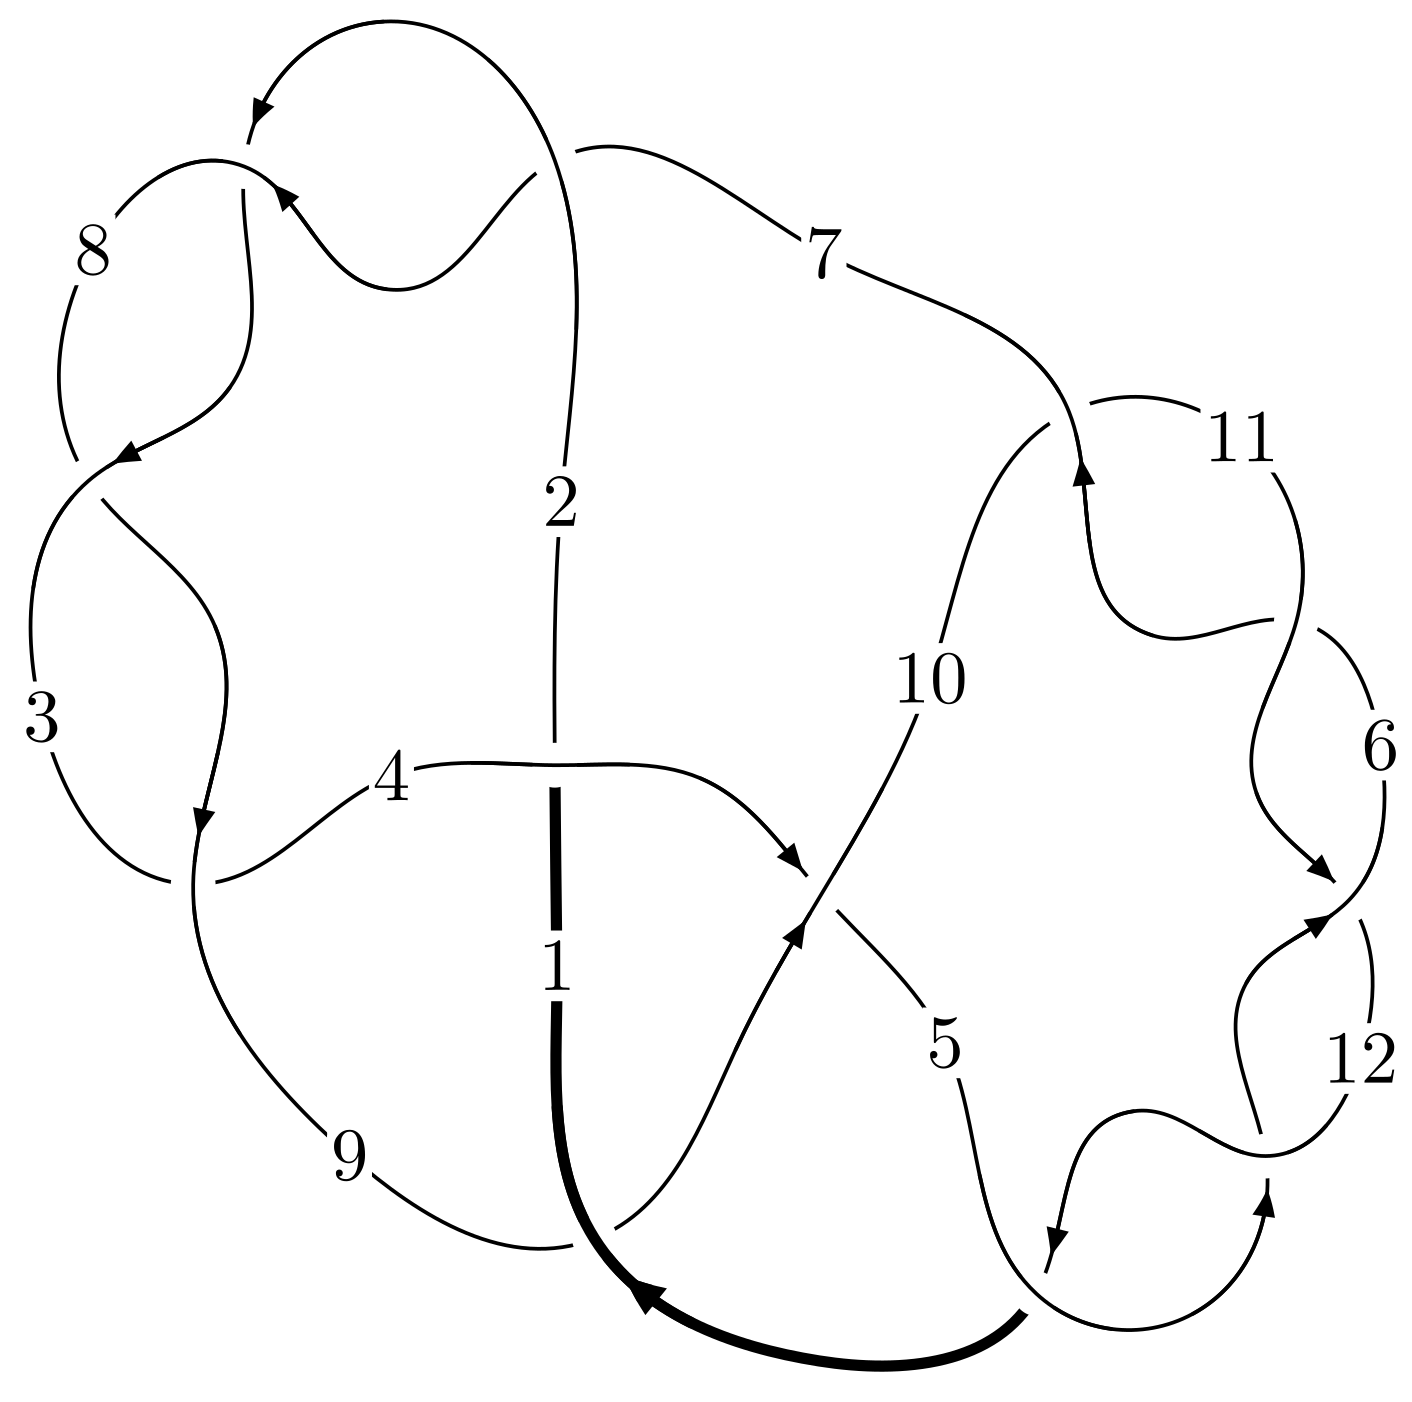
\includegraphics[width=112pt]{../../../GIT/diagram.site/Diagrams/png/1939_12a_1138.png}\\
\ \ \ A knot diagram\footnotemark}&
\allowdisplaybreaks
\textbf{Linearized knot diagam} \\
\cline{2-2}
 &
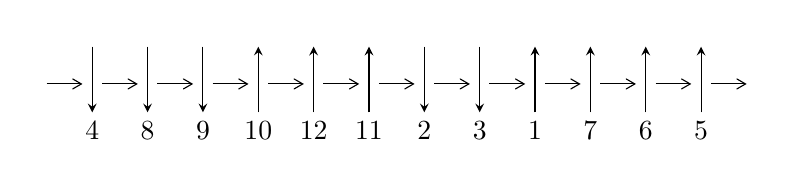
\begin{tikzpicture}[x=20pt, y=17pt]
	% nodes
	\node (C0) at (0, 0) {};
	\node (C1) at (1, 0) {};
	\node (C1U) at (1, +1) {};
	\node (C1D) at (1, -1) {4};

	\node (C2) at (2, 0) {};
	\node (C2U) at (2, +1) {};
	\node (C2D) at (2, -1) {8};

	\node (C3) at (3, 0) {};
	\node (C3U) at (3, +1) {};
	\node (C3D) at (3, -1) {9};

	\node (C4) at (4, 0) {};
	\node (C4U) at (4, +1) {};
	\node (C4D) at (4, -1) {10};

	\node (C5) at (5, 0) {};
	\node (C5U) at (5, +1) {};
	\node (C5D) at (5, -1) {12};

	\node (C6) at (6, 0) {};
	\node (C6U) at (6, +1) {};
	\node (C6D) at (6, -1) {11};

	\node (C7) at (7, 0) {};
	\node (C7U) at (7, +1) {};
	\node (C7D) at (7, -1) {2};

	\node (C8) at (8, 0) {};
	\node (C8U) at (8, +1) {};
	\node (C8D) at (8, -1) {3};

	\node (C9) at (9, 0) {};
	\node (C9U) at (9, +1) {};
	\node (C9D) at (9, -1) {1};

	\node (C10) at (10, 0) {};
	\node (C10U) at (10, +1) {};
	\node (C10D) at (10, -1) {7};

	\node (C11) at (11, 0) {};
	\node (C11U) at (11, +1) {};
	\node (C11D) at (11, -1) {6};

	\node (C12) at (12, 0) {};
	\node (C12U) at (12, +1) {};
	\node (C12D) at (12, -1) {5};
	\node (C13) at (13, 0) {};

	% arrows
	\draw[->,>={angle 60}]
	(C0) edge (C1) (C1) edge (C2) (C2) edge (C3) (C3) edge (C4) (C4) edge (C5) (C5) edge (C6) (C6) edge (C7) (C7) edge (C8) (C8) edge (C9) (C9) edge (C10) (C10) edge (C11) (C11) edge (C12) (C12) edge (C13) ;	\draw[->,>=stealth]
	(C1U) edge (C1D) (C2U) edge (C2D) (C3U) edge (C3D) (C4D) edge (C4U) (C5D) edge (C5U) (C6D) edge (C6U) (C7U) edge (C7D) (C8U) edge (C8D) (C9D) edge (C9U) (C10D) edge (C10U) (C11D) edge (C11U) (C12D) edge (C12U) ;
	\end{tikzpicture} \\
\hhline{~~} \\& 
\textbf{Solving Sequence} \\ \cline{2-2} 
 &
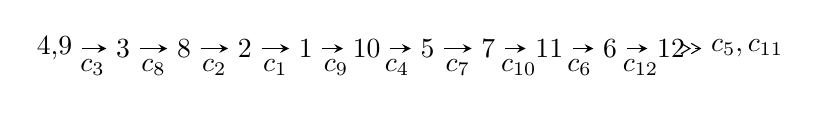
\begin{tikzpicture}[x=22pt, y=7pt]
	% node
	\node (A0) at (-1/8, 0) {4,9};
	\node (A1) at (1, 0) {3};
	\node (A2) at (2, 0) {8};
	\node (A3) at (3, 0) {2};
	\node (A4) at (4, 0) {1};
	\node (A5) at (5, 0) {10};
	\node (A6) at (6, 0) {5};
	\node (A7) at (7, 0) {7};
	\node (A8) at (8, 0) {11};
	\node (A9) at (9, 0) {6};
	\node (A10) at (10, 0) {12};
	\node (C1) at (1/2, -1) {$c_{3}$};
	\node (C2) at (3/2, -1) {$c_{8}$};
	\node (C3) at (5/2, -1) {$c_{2}$};
	\node (C4) at (7/2, -1) {$c_{1}$};
	\node (C5) at (9/2, -1) {$c_{9}$};
	\node (C6) at (11/2, -1) {$c_{4}$};
	\node (C7) at (13/2, -1) {$c_{7}$};
	\node (C8) at (15/2, -1) {$c_{10}$};
	\node (C9) at (17/2, -1) {$c_{6}$};
	\node (C10) at (19/2, -1) {$c_{12}$};
	\node (A11) at (45/4, 0) {$c_{5},c_{11}$};

	% edge
	\draw[->,>=stealth]	
	(A0) edge (A1) (A1) edge (A2) (A2) edge (A3) (A3) edge (A4) (A4) edge (A5) (A5) edge (A6) (A6) edge (A7) (A7) edge (A8) (A8) edge (A9) (A9) edge (A10) ;
	\draw[->>,>={angle 60}]	
	(A10) edge (A11);
\end{tikzpicture} \\ 

\end{tabular} \\

\footnotetext{
The image of knot diagram is generated by the software ``\textbf{Draw programme}" developed by Andrew Bartholomew(\url{http://www.layer8.co.uk/maths/draw/index.htm\#Running-draw}), where we modified some parts for our purpose(\url{https://github.com/CATsTAILs/LinksPainter}).
}\phantom \\ \newline 
\centering \textbf{Ideals for irreducible components\footnotemark of $X_{\text{par}}$} 
 
\begin{align*}
I^u_{1}&=\langle 
u^{39}- u^{38}+\cdots+4 u^3-1\rangle \\
\\
\end{align*}
\raggedright * 1 irreducible components of $\dim_{\mathbb{C}}=0$, with total 39 representations.\\
\footnotetext{All coefficients of polynomials are rational numbers. But the coefficients are sometimes approximated in decimal forms when there is not enough margin.}
\newpage
\renewcommand{\arraystretch}{1}
\centering \section*{I. $I^u_{1}= \langle u^{39}- u^{38}+\cdots+4 u^3-1 \rangle$}
\flushleft \textbf{(i) Arc colorings}\\
\begin{tabular}{m{7pt} m{180pt} m{7pt} m{180pt} }
\flushright $a_{4}=$&$\begin{pmatrix}1\\0\end{pmatrix}$ \\
\flushright $a_{9}=$&$\begin{pmatrix}0\\u\end{pmatrix}$ \\
\flushright $a_{3}=$&$\begin{pmatrix}1\\- u^2\end{pmatrix}$ \\
\flushright $a_{8}=$&$\begin{pmatrix}u\\- u^3+u\end{pmatrix}$ \\
\flushright $a_{2}=$&$\begin{pmatrix}- u^2+1\\u^4-2 u^2\end{pmatrix}$ \\
\flushright $a_{1}=$&$\begin{pmatrix}u^4-3 u^2+1\\u^4-2 u^2\end{pmatrix}$ \\
\flushright $a_{10}=$&$\begin{pmatrix}u^9-6 u^7+11 u^5-6 u^3+u\\u^9-5 u^7+7 u^5-2 u^3+u\end{pmatrix}$ \\
\flushright $a_{5}=$&$\begin{pmatrix}- u^{18}+11 u^{16}-48 u^{14}+105 u^{12}-121 u^{10}+75 u^8-30 u^6+8 u^4- u^2+1\\- u^{18}+10 u^{16}-39 u^{14}+74 u^{12}-71 u^{10}+38 u^8-18 u^6+4 u^4- u^2\end{pmatrix}$ \\
\flushright $a_{7}=$&$\begin{pmatrix}- u^3+2 u\\u^5-3 u^3+u\end{pmatrix}$ \\
\flushright $a_{11}=$&$\begin{pmatrix}u^{17}-10 u^{15}+39 u^{13}-74 u^{11}+71 u^9-38 u^7+18 u^5-4 u^3+u\\- u^{19}+11 u^{17}-48 u^{15}+105 u^{13}-121 u^{11}+75 u^9-30 u^7+8 u^5- u^3+u\end{pmatrix}$ \\
\flushright $a_{6}=$&$\begin{pmatrix}- u^{31}+18 u^{29}+\cdots-12 u^7+2 u\\u^{33}-19 u^{31}+\cdots-2 u^3+u\end{pmatrix}$ \\
\flushright $a_{12}=$&$\begin{pmatrix}u^{32}-19 u^{30}+\cdots-2 u^2+1\\u^{32}-18 u^{30}+\cdots+12 u^8-2 u^2\end{pmatrix}$\\&\end{tabular}
\flushleft \textbf{(ii) Obstruction class $= -1$}\\~\\
\flushleft \textbf{(iii) Cusp Shapes $= 4 u^{36}-84 u^{34}+788 u^{32}+4 u^{31}-4352 u^{30}-72 u^{29}+15712 u^{28}+568 u^{27}-38992 u^{26}-2576 u^{25}+68272 u^{24}+7412 u^{23}-85520 u^{22}-14120 u^{21}+77072 u^{20}+18120 u^{19}-49428 u^{18}-15728 u^{17}+21212 u^{16}+9112 u^{15}-4912 u^{14}-3220 u^{13}-12 u^{12}+432 u^{11}+284 u^{10}+36 u^9+88 u^8+52 u^7-84 u^6-64 u^5+44 u^4+20 u^3-4 u^2-4 u+2$}\\~\\
\newpage\renewcommand{\arraystretch}{1}
\flushleft \textbf{(iv) u-Polynomials at the component}\newline \\
\begin{tabular}{m{50pt}|m{274pt}}
Crossings & \hspace{64pt}u-Polynomials at each crossing \\
\hline $$\begin{aligned}c_{1}\end{aligned}$$&$\begin{aligned}
&u^{39}-11 u^{38}+\cdots+360 u-41
\end{aligned}$\\
\hline $$\begin{aligned}c_{2},c_{3},c_{7}\\c_{8}\end{aligned}$$&$\begin{aligned}
&u^{39}+u^{38}+\cdots+4 u^3+1
\end{aligned}$\\
\hline $$\begin{aligned}c_{4}\end{aligned}$$&$\begin{aligned}
&u^{39}- u^{38}+\cdots+112 u+29
\end{aligned}$\\
\hline $$\begin{aligned}c_{5},c_{6},c_{10}\\c_{11},c_{12}\end{aligned}$$&$\begin{aligned}
&u^{39}- u^{38}+\cdots-2 u+1
\end{aligned}$\\
\hline $$\begin{aligned}c_{9}\end{aligned}$$&$\begin{aligned}
&u^{39}-5 u^{38}+\cdots+112 u-95
\end{aligned}$\\
\hline
\end{tabular}\\~\\
\newpage\renewcommand{\arraystretch}{1}
\flushleft \textbf{(v) Riley Polynomials at the component}\newline \\
\begin{tabular}{m{50pt}|m{274pt}}
Crossings & \hspace{64pt}Riley Polynomials at each crossing \\
\hline $$\begin{aligned}c_{1}\end{aligned}$$&$\begin{aligned}
&y^{39}-9 y^{38}+\cdots+3156 y-1681
\end{aligned}$\\
\hline $$\begin{aligned}c_{2},c_{3},c_{7}\\c_{8}\end{aligned}$$&$\begin{aligned}
&y^{39}-45 y^{38}+\cdots-10 y^2-1
\end{aligned}$\\
\hline $$\begin{aligned}c_{4}\end{aligned}$$&$\begin{aligned}
&y^{39}+11 y^{38}+\cdots+5352 y-841
\end{aligned}$\\
\hline $$\begin{aligned}c_{5},c_{6},c_{10}\\c_{11},c_{12}\end{aligned}$$&$\begin{aligned}
&y^{39}+51 y^{38}+\cdots-2 y^2-1
\end{aligned}$\\
\hline $$\begin{aligned}c_{9}\end{aligned}$$&$\begin{aligned}
&y^{39}+19 y^{38}+\cdots-71816 y-9025
\end{aligned}$\\
\hline
\end{tabular}\\~\\
\newpage\flushleft \textbf{(vi) Complex Volumes and Cusp Shapes}
$$\begin{array}{c|c|c}  
\text{Solutions to }I^u_{1}& \I (\text{vol} + \sqrt{-1}CS) & \text{Cusp shape}\\
 \hline 
\begin{aligned}
u &= \phantom{-}0.841792 + 0.292424 I\end{aligned}
 & -15.1182 + 1.5057 I & -8.40858 + 0.97265 I \\ \hline\begin{aligned}
u &= \phantom{-}0.841792 - 0.292424 I\end{aligned}
 & -15.1182 - 1.5057 I & -8.40858 - 0.97265 I \\ \hline\begin{aligned}
u &= -0.729257 + 0.492469 I\end{aligned}
 & -13.7612 + 8.1189 I & -6.01582 - 6.71736 I \\ \hline\begin{aligned}
u &= -0.729257 - 0.492469 I\end{aligned}
 & -13.7612 - 8.1189 I & -6.01582 + 6.71736 I \\ \hline\begin{aligned}
u &= \phantom{-}0.707989 + 0.470053 I\end{aligned}
 & -4.12575 - 6.63014 I & -5.12153 + 8.45771 I \\ \hline\begin{aligned}
u &= \phantom{-}0.707989 - 0.470053 I\end{aligned}
 & -4.12575 + 6.63014 I & -5.12153 - 8.45771 I \\ \hline\begin{aligned}
u &= -0.774155 + 0.278442 I\end{aligned}
 & -5.35026 - 0.56012 I & -8.31402 - 0.25589 I \\ \hline\begin{aligned}
u &= -0.774155 - 0.278442 I\end{aligned}
 & -5.35026 + 0.56012 I & -8.31402 + 0.25589 I \\ \hline\begin{aligned}
u &= -0.668788 + 0.436144 I\end{aligned}
 & -0.40953 + 3.91689 I & \phantom{-}0.46864 - 8.35859 I \\ \hline\begin{aligned}
u &= -0.668788 - 0.436144 I\end{aligned}
 & -0.40953 - 3.91689 I & \phantom{-}0.46864 + 8.35859 I \\ \hline\begin{aligned}
u &= \phantom{-}0.635570 + 0.340805 I\end{aligned}
 & -1.13161 - 1.10437 I & -2.87714 + 0.84766 I \\ \hline\begin{aligned}
u &= \phantom{-}0.635570 - 0.340805 I\end{aligned}
 & -1.13161 + 1.10437 I & -2.87714 - 0.84766 I \\ \hline\begin{aligned}
u &= -0.451697 + 0.506497 I\end{aligned}
 & -9.02178 + 1.76146 I & -1.28786 - 3.92479 I \\ \hline\begin{aligned}
u &= -0.451697 - 0.506497 I\end{aligned}
 & -9.02178 - 1.76146 I & -1.28786 + 3.92479 I \\ \hline\begin{aligned}
u &= -0.136161 + 0.598793 I\end{aligned}
 & -12.02260 - 4.41211 I & -2.43306 + 1.96254 I \\ \hline\begin{aligned}
u &= -0.136161 - 0.598793 I\end{aligned}
 & -12.02260 + 4.41211 I & -2.43306 - 1.96254 I \\ \hline\begin{aligned}
u &= \phantom{-}0.143045 + 0.548355 I\end{aligned}
 & -2.49224 + 3.13322 I & -1.35770 - 3.51211 I \\ \hline\begin{aligned}
u &= \phantom{-}0.143045 - 0.548355 I\end{aligned}
 & -2.49224 - 3.13322 I & -1.35770 + 3.51211 I \\ \hline\begin{aligned}
u &= \phantom{-}0.394285 + 0.400255 I\end{aligned}
 & -0.58188 - 1.38142 I & -0.08240 + 6.03363 I \\ \hline\begin{aligned}
u &= \phantom{-}0.394285 - 0.400255 I\end{aligned}
 & -0.58188 + 1.38142 I & -0.08240 - 6.03363 I \\ \hline\begin{aligned}
u &= \phantom{-}1.49254\phantom{ +0.000000I}\end{aligned}
 & -4.41211\phantom{ +0.000000I} & \phantom{-0.000000 } 0 \\ \hline\begin{aligned}
u &= \phantom{-}1.49483 + 0.09365 I\end{aligned}
 & -15.3639 - 3.7798 I & \phantom{-0.000000 } 0 \\ \hline\begin{aligned}
u &= \phantom{-}1.49483 - 0.09365 I\end{aligned}
 & -15.3639 + 3.7798 I & \phantom{-0.000000 } 0 \\ \hline\begin{aligned}
u &= -1.50080 + 0.04783 I\end{aligned}
 & -6.77867 + 2.73633 I & \phantom{-0.000000 } 0 \\ \hline\begin{aligned}
u &= -1.50080 - 0.04783 I\end{aligned}
 & -6.77867 - 2.73633 I & \phantom{-0.000000 } 0 \\ \hline\begin{aligned}
u &= -0.196225 + 0.449165 I\end{aligned}
 & \phantom{-}0.943197 - 0.763976 I & \phantom{-}6.20859 + 2.38716 I \\ \hline\begin{aligned}
u &= -0.196225 - 0.449165 I\end{aligned}
 & \phantom{-}0.943197 + 0.763976 I & \phantom{-}6.20859 - 2.38716 I \\ \hline\begin{aligned}
u &= -1.59322 + 0.10217 I\end{aligned}
 & -8.77741 + 2.76966 I & \phantom{-0.000000 } 0 \\ \hline\begin{aligned}
u &= -1.59322 - 0.10217 I\end{aligned}
 & -8.77741 - 2.76966 I & \phantom{-0.000000 } 0 \\ \hline\begin{aligned}
u &= \phantom{-}1.59721 + 0.12385 I\end{aligned}
 & -8.12235 - 5.98293 I & \phantom{-0.000000 } 0\\
 \hline 
 \end{array}$$\newpage$$\begin{array}{c|c|c}  
\text{Solutions to }I^u_{1}& \I (\text{vol} + \sqrt{-1}CS) & \text{Cusp shape}\\
 \hline 
\begin{aligned}
u &= \phantom{-}1.59721 - 0.12385 I\end{aligned}
 & -8.12235 + 5.98293 I & \phantom{-0.000000 } 0 \\ \hline\begin{aligned}
u &= -1.60787 + 0.13573 I\end{aligned}
 & -11.9998 + 8.8902 I & \phantom{-0.000000 } 0 \\ \hline\begin{aligned}
u &= -1.60787 - 0.13573 I\end{aligned}
 & -11.9998 - 8.8902 I & \phantom{-0.000000 } 0 \\ \hline\begin{aligned}
u &= \phantom{-}1.61669 + 0.08086 I\end{aligned}
 & -13.52220 - 0.80582 I & \phantom{-0.000000 } 0 \\ \hline\begin{aligned}
u &= \phantom{-}1.61669 - 0.08086 I\end{aligned}
 & -13.52220 + 0.80582 I & \phantom{-0.000000 } 0 \\ \hline\begin{aligned}
u &= \phantom{-}1.61512 + 0.14352 I\end{aligned}
 & \phantom{-}17.7470 - 10.5062 I & \phantom{-0.000000 } 0 \\ \hline\begin{aligned}
u &= \phantom{-}1.61512 - 0.14352 I\end{aligned}
 & \phantom{-}17.7470 + 10.5062 I & \phantom{-0.000000 } 0 \\ \hline\begin{aligned}
u &= -1.63463 + 0.07714 I\end{aligned}
 & \phantom{-}15.8667 - 0.1255 I & \phantom{-0.000000 } 0 \\ \hline\begin{aligned}
u &= -1.63463 - 0.07714 I\end{aligned}
 & \phantom{-}15.8667 + 0.1255 I & \phantom{-0.000000 } 0\\
 \hline 
 \end{array}$$\newpage
\newpage\renewcommand{\arraystretch}{1}
\centering \section*{ II. u-Polynomials}
\begin{tabular}{m{50pt}|m{274pt}}
Crossings & \hspace{64pt}u-Polynomials at each crossing \\
\hline $$\begin{aligned}c_{1}\end{aligned}$$&$\begin{aligned}
&u^{39}-11 u^{38}+\cdots+360 u-41
\end{aligned}$\\
\hline $$\begin{aligned}c_{2},c_{3},c_{7}\\c_{8}\end{aligned}$$&$\begin{aligned}
&u^{39}+u^{38}+\cdots+4 u^3+1
\end{aligned}$\\
\hline $$\begin{aligned}c_{4}\end{aligned}$$&$\begin{aligned}
&u^{39}- u^{38}+\cdots+112 u+29
\end{aligned}$\\
\hline $$\begin{aligned}c_{5},c_{6},c_{10}\\c_{11},c_{12}\end{aligned}$$&$\begin{aligned}
&u^{39}- u^{38}+\cdots-2 u+1
\end{aligned}$\\
\hline $$\begin{aligned}c_{9}\end{aligned}$$&$\begin{aligned}
&u^{39}-5 u^{38}+\cdots+112 u-95
\end{aligned}$\\
\hline
\end{tabular}\newpage\renewcommand{\arraystretch}{1}
\centering \section*{ III. Riley Polynomials}
\begin{tabular}{m{50pt}|m{274pt}}
Crossings & \hspace{64pt}Riley Polynomials at each crossing \\
\hline $$\begin{aligned}c_{1}\end{aligned}$$&$\begin{aligned}
&y^{39}-9 y^{38}+\cdots+3156 y-1681
\end{aligned}$\\
\hline $$\begin{aligned}c_{2},c_{3},c_{7}\\c_{8}\end{aligned}$$&$\begin{aligned}
&y^{39}-45 y^{38}+\cdots-10 y^2-1
\end{aligned}$\\
\hline $$\begin{aligned}c_{4}\end{aligned}$$&$\begin{aligned}
&y^{39}+11 y^{38}+\cdots+5352 y-841
\end{aligned}$\\
\hline $$\begin{aligned}c_{5},c_{6},c_{10}\\c_{11},c_{12}\end{aligned}$$&$\begin{aligned}
&y^{39}+51 y^{38}+\cdots-2 y^2-1
\end{aligned}$\\
\hline $$\begin{aligned}c_{9}\end{aligned}$$&$\begin{aligned}
&y^{39}+19 y^{38}+\cdots-71816 y-9025
\end{aligned}$\\
\hline
\end{tabular}
\vskip 2pc
\end{document}